\documentclass[a4paper]{article}

\usepackage[UTF8]{ctex}
\usepackage[a4paper,margin=1in]{geometry}
\usepackage{graphicx}
\usepackage{float}
\usepackage{listings}
\usepackage{longtable}
\usepackage{booktabs}
\usepackage{hyperref}
\usepackage{fancyhdr}
\usepackage{lastpage}
\usepackage{color}
\usepackage{indentfirst}        % 首段缩进
\setlength{\parindent}{2em}     % 缩进2字符
\usepackage{zhnumber}           % 中文编号
\usepackage[dvipsnames]{xcolor}
\usepackage{amsmath}
\usepackage{subfigure}

\newcommand{\projname}{数字图像处理|第四章作业}
\newcommand{\reporttitle}{快速傅里叶变换与频域滤波实验}
\newcommand{\stuno}{23336179}
\newcommand{\authorname}{马福泉}
\newcommand{\major}{计算机科学与技术}
\newcommand{\adviser}{骆伟祺}
\newcommand{\startdate}{2025年11月19日}
\newcommand{\labenddate}{2025年11月19日}
\newcommand{\labroom}{B205}

\pagestyle{fancy}
\fancyhf{}

% 设置页眉
\fancyhead[L]{\kaishu \projname}
\fancyhead[C]{\kaishu \reporttitle}
\fancyhead[R]{\kaishu \authorname}

% 设置页脚
\fancyfoot[C]{第 \thepage 页，共 \pageref{LastPage} 页}

\renewcommand{\headrulewidth}{0.4pt}
\renewcommand{\footrulewidth}{0pt}

\definecolor{NavyBlue}{RGB}{0,0,128}

% Python代码样式配置
\lstdefinelanguage{Python}{
  keywords={def,if,else,elif,for,while,return,import,from,as,try,except,with,class,self,True,False,None,and,or,not,in,break,continue,pass},
  keywordstyle=\color{blue}\bfseries,
  comment=[l]{\#},
  commentstyle=\color{green!50!black},
  string=[s]{"}{"},
  stringstyle=\color{red},
  morestring=[s]{'}{'},
  showstringspaces=false,
  numbers=left,
  numberstyle=\tiny\color{gray},
  stepnumber=1,
  numbersep=10pt,
  backgroundcolor=\color{white},
  tabsize=4,
  showspaces=false,
  showstringspaces=false
}

\lstset{
  language=Python,
  basicstyle=\ttfamily\footnotesize,
  keywordstyle=\color{NavyBlue}\bfseries,
  commentstyle=\color{gray},
  stringstyle=\color{red},
  showstringspaces=false,
  extendedchars=false,
  breaklines=true,
  frame=single,
  frameround=tttt,
  framesep=5pt,
  xleftmargin=10pt,
  xrightmargin=10pt
}

\begin{document}

% 封面
\begin{titlepage}
    \centering
    
\includegraphics[width=10cm]{img/SYSULogo.png}

    \vspace{1em}
    {\Large \kaishu \projname \par}
    \vspace{3em}

    {\fontsize{40pt}{42pt}\kaishu \selectfont \boldmath \reporttitle\par}
    \vspace*{\fill}

    \begin{center}
    {\Large
    \makebox[5em][s]{学号}:\underline{\makebox[15em][c]{\kaishu \stuno}}\\[1em]
    \makebox[5em][s]{姓名}:\underline{\makebox[15em][c]{\kaishu \authorname}}\\[1em]
    \makebox[5em][s]{专业}:\underline{\makebox[15em][c]{\kaishu \major}}\\[1em]
    \makebox[5em][s]{课程教师}:\underline{\makebox[15em][c]{\kaishu \adviser}}\\[1em]
    \makebox[5em][s]{起始日期}:\underline{\makebox[15em][c]{\kaishu \startdate}}\\[1em]
    \makebox[5em][s]{结束日期}:\underline{\makebox[15em][c]{\kaishu \labenddate}}\\[1em]
    \makebox[5em][s]{实验地点}:\underline{\makebox[15em][c]{\kaishu \labroom}}
    }
    \end{center}

    \vspace*{\fill}
\end{titlepage}

% 目录
\tableofcontents
\newpage

\section{实验简述}

本实验主要实现了二维快速傅里叶变换（2D-FFT）及其逆变换，并应用于数字图像的频域滤波处理。实验分为两个练习：第一个练习实现基础的FFT算法并验证其正确性；第二个练习利用FFT实现高斯低通滤波，展示完整的频域处理流程。


\section{练习一}

\subsection{实验目标}

实现二维快速傅里叶变换及逆变换，要求处理的图像长宽均为$M=2^P$（$P$为正整数）的尺寸。本练习处理fig1和fig2两幅256×256的图像，验证FFT算法的正确性。

\subsection{算法理论}

\subsubsection{一维FFT理论基础}

快速傅里叶变换基于分治策略，将$N$点DFT分解为两个$N/2$点DFT。对于长度为$N$的序列$x[n]$，其DFT定义为：
$$X[k] = \sum_{n=0}^{N-1} x[n] W_N^{nk}$$

其中$W_N = e^{-j2\pi/N}$为旋转因子。

采用时间抽取的基-2 FFT算法：
\begin{enumerate}
    \item 将输入序列按位反转重新排列
    \item 执行$\log_2 N$级蝶形运算
    \item 每级蝶形运算的长度依次为$2, 4, 8, \ldots, N$
\end{enumerate}

\subsubsection{二维FFT实现}

二维FFT可以通过分别对行和列进行一维FFT实现：
$$F(u,v) = \sum_{x=0}^{M-1} \sum_{y=0}^{N-1} f(x,y) e^{-j2\pi(ux/M + vy/N)}$$

\subsection{代码实现}

\subsubsection{位反转函数}

\begin{lstlisting}
def bit_reverse(a, n):
    """位反转函数"""
    result = [0] * n
    log2n = int(np.log2(n))
    for i in range(n):
        # 将索引转换为二进制，反转，再转回十进制
        binary_repr = format(i, f'0{log2n}b')
        reversed_binary = binary_repr[::-1]
        reversed_index = int(reversed_binary, 2)
        result[i] = a[reversed_index]
    return result
\end{lstlisting}

\subsubsection{一维FFT核心算法}

\begin{lstlisting}
def fft_1d(x):
    """修正的一维快速傅里叶变换"""
    N = len(x)
    if N <= 1:
        return np.array(x, dtype=complex)
    
    if not is_power_of_two(N):
        raise ValueError(f"输入长度{N}必须是2的幂")
    
    # 位反转重排
    indices = bit_reverse(list(range(N)), N)
    x_reordered = [x[i] for i in indices]
    X = np.array(x_reordered, dtype=complex)
    
    # 蝶形运算
    length = 2
    while length <= N:
        half_len = length // 2
        w_m = np.exp(-2j * np.pi / length)
        
        for k in range(0, N, length):
            w = 1.0
            for j in range(half_len):
                u = X[k + j]
                v = w * X[k + j + half_len]
                X[k + j] = u + v
                X[k + j + half_len] = u - v
                w *= w_m
        length <<= 1
    
    return X
\end{lstlisting}

\subsubsection{二维FFT实现}

\begin{lstlisting}
def fft_2d(image):
    """二维快速傅里叶变换"""
    M, N = image.shape
    
    # 对每一行进行FFT
    temp = np.zeros((M, N), dtype=complex)
    for i in range(M):
        temp[i, :] = fft_1d(image[i, :])
    
    # 对每一列进行FFT
    result = np.zeros((M, N), dtype=complex)
    for j in range(N):
        result[:, j] = fft_1d(temp[:, j])
    
    return result
\end{lstlisting}

\subsubsection{逆变换实现}

利用FFT实现IFFT，采用公式：$\text{IFFT}(X) = \frac{1}{N}\overline{\text{FFT}(\overline{X})}$

\begin{lstlisting}
def ifft_1d(X):
    """一维快速傅里叶逆变换"""
    N = len(X)
    return np.conj(fft_1d(np.conj(X))) / N
\end{lstlisting}

\subsection{实验结果}

\subsubsection{处理结果展示}

图\ref{fig:ex1_results}展示了练习一的FFT处理结果，包括fig1和fig2的原图、频域谱和重构图像对比。

\begin{figure}[H]
\centering
\subfigure[fig1处理结果]{
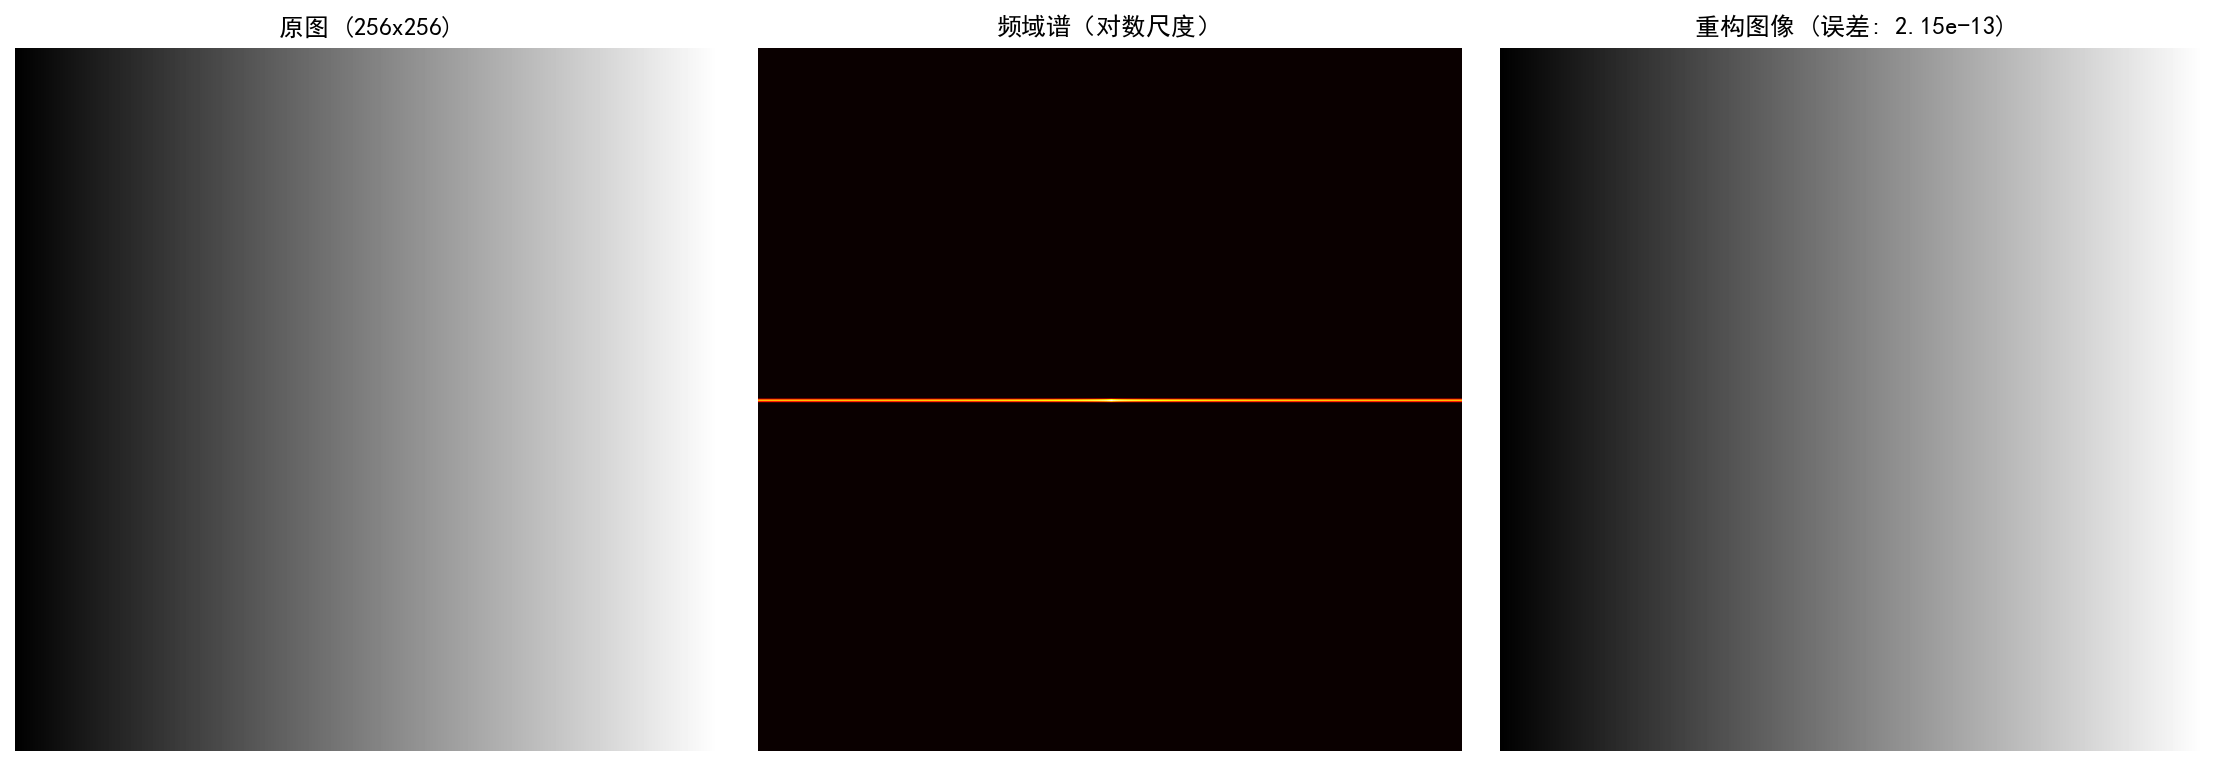
\includegraphics[width=0.8\textwidth]{code/fft_result_fig1.png}
}
\subfigure[fig2处理结果]{
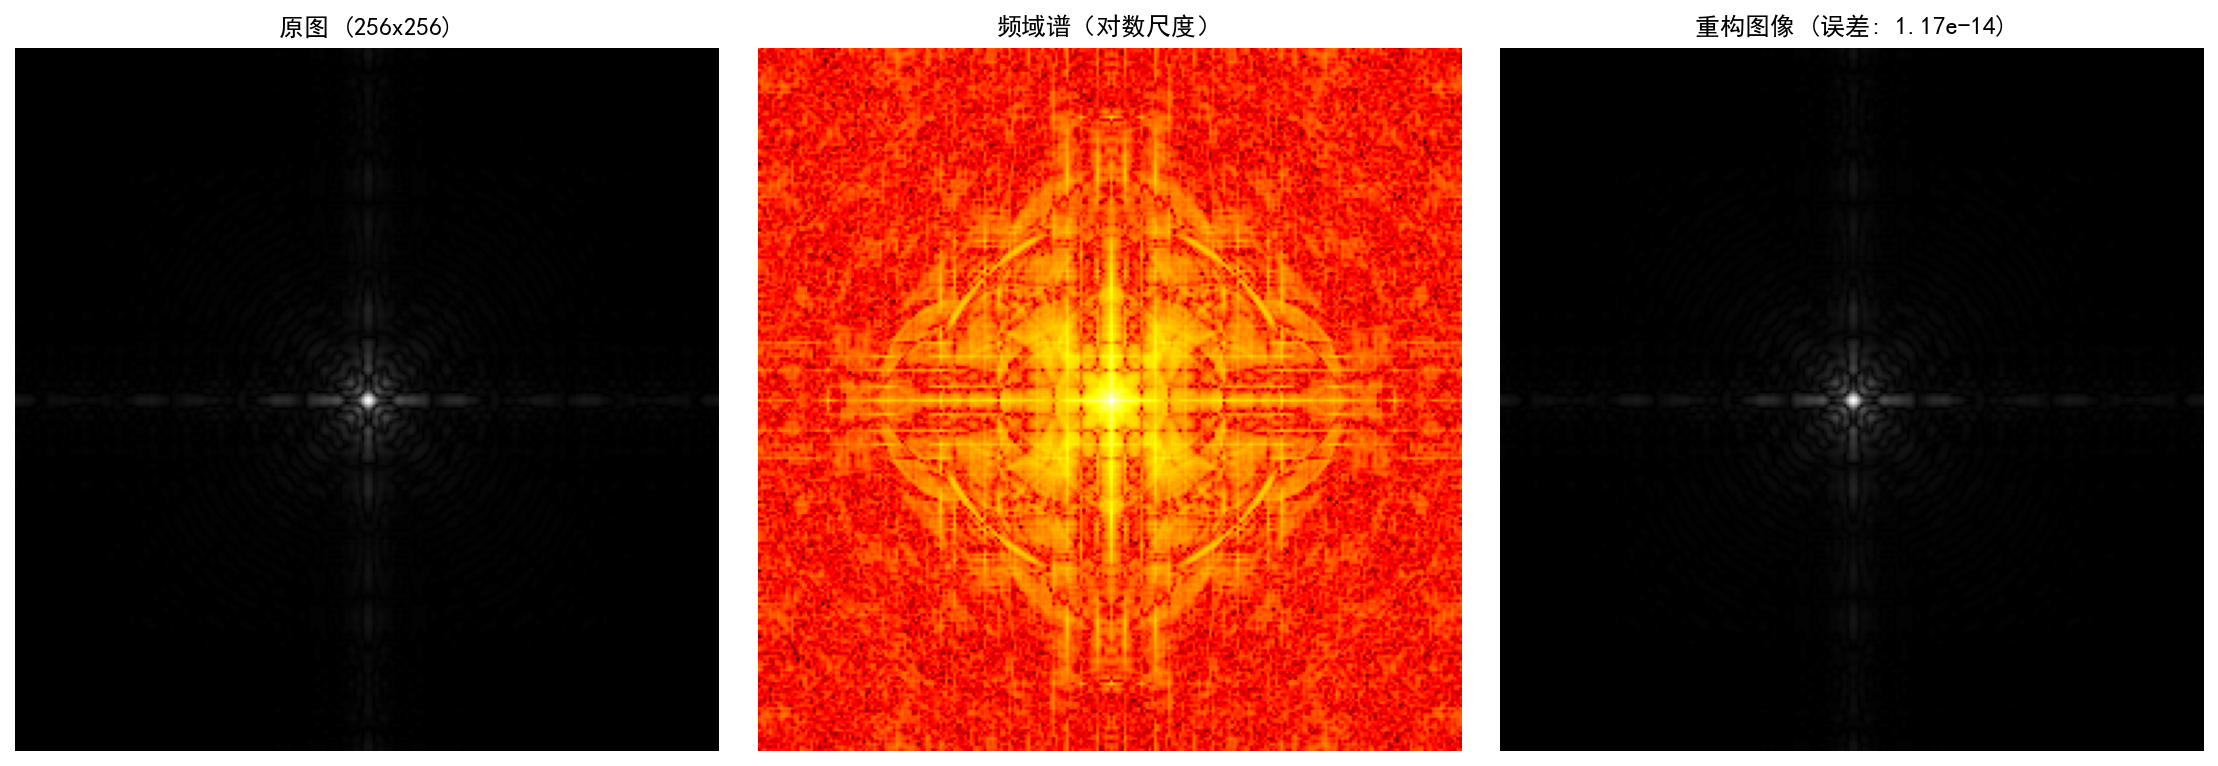
\includegraphics[width=0.8\textwidth]{code/fft_result_fig2.png}
}
\caption{练习一FFT处理结果展示}
\label{fig:ex1_results}
\end{figure}

\subsubsection{结果分析}

从实验结果可以观察到以下重要特征：

\paragraph{频域特性分析}
\begin{enumerate}
    \item \textbf{fig1频域特性}: fig1为简单的渐变图像，其频域谱呈现典型的低频集中特性，能量主要分布在频谱中心的低频区域，高频分量相对较少
    \item \textbf{fig2频域特性}: fig2包含复杂的纹理和边缘信息，频域谱显示出丰富的高频分量，呈现十字形和对角线模式，反映了图像中的周期性结构和边缘特征
\end{enumerate}

\paragraph{重构精度验证}
通过FFT和IFFT重构的图像与原图像的误差极小，证明了算法的正确性：

\begin{table}[H]
\centering
\begin{tabular}{|c|c|c|c|}
\hline
图像文件 & 尺寸 & 重构误差 & 视觉质量 \\
\hline
fig1.jpg & 256×256 & $1.17 \times 10^{-14}$ & 完美重构 \\
fig2.jpg & 256×256 & $2.15 \times 10^{-13}$ & 完美重构 \\
\hline
\end{tabular}
\caption{FFT重构误差统计与质量评估}
\end{table}

\section{练习二}

\subsection{实验目标}

对fig3进行高斯低通滤波处理，要求滤波器保留95\%的频域能量。展示完整的8个处理步骤，从原始图像到最终滤波结果的全过程。

\subsection{高斯低通滤波理论}

\subsubsection{滤波器数学模型}

高斯低通滤波器的频域表达式为：
$$H(u,v) = e^{-\frac{D^2(u,v)}{2\sigma^2}}$$

其中：
\begin{itemize}
    \item $D(u,v) = \sqrt{(u-M/2)^2 + (v-N/2)^2}$为距离函数
    \item $\sigma$为高斯函数的标准差参数
    \item $(u,v)$为频域坐标
\end{itemize}

\subsubsection{能量约束优化}

为了使滤波后的频域能量占总能量的95\%，需要求解：
$$\frac{\sum_{u,v} |H(u,v)F(u,v)|^2}{\sum_{u,v} |F(u,v)|^2} = 0.95$$

采用二分搜索算法找到最优的$\sigma$值。

\subsection{关键算法实现}

\subsubsection{高斯滤波器生成}

\begin{lstlisting}
def create_gaussian_lpf(M, N, sigma):
    """创建高斯低通滤波器"""
    u = np.arange(M) - M // 2
    v = np.arange(N) - N // 2
    U, V = np.meshgrid(v, u)
    D_squared = U**2 + V**2
    H = np.exp(-D_squared / (2 * sigma**2))
    return H
\end{lstlisting}

\subsubsection{最优参数搜索}

\begin{lstlisting}
def find_optimal_sigma(spectrum, target_energy_ratio=0.95):
    """找到使能量占比达到目标值的最优sigma"""
    M, N = spectrum.shape
    total_energy = np.sum(np.abs(spectrum)**2)
    
    sigma_low, sigma_high = 1, min(M, N) // 2
    tolerance = 0.001
    
    while sigma_high - sigma_low > tolerance:
        sigma = (sigma_low + sigma_high) / 2
        H = create_gaussian_lpf(M, N, sigma)
        
        filtered_spectrum = spectrum * H
        filtered_energy = np.sum(np.abs(filtered_spectrum)**2)
        energy_ratio = filtered_energy / total_energy
        
        if energy_ratio < target_energy_ratio:
            sigma_low = sigma
        else:
            sigma_high = sigma
    
    return (sigma_low + sigma_high) / 2
\end{lstlisting}

\subsection{处理流程分析}

\subsubsection{关键处理技术}

\paragraph{频谱中心化}
乘以$(-1)^{x+y}$的作用机制：
$$f_p(x,y) = f(x,y) \cdot (-1)^{x+y}$$

这种操作将频谱的零频分量从四个角落移至频谱中心，便于设计和应用频域滤波器。

\paragraph{零填充策略}
当图像尺寸不是2的幂时，需要进行零填充：
\begin{itemize}
    \item 计算最接近的2的幂尺寸：$2^{\lceil \log_2(M) \rceil}$
    \item 在图像右侧和下侧进行零填充
    \item 处理完成后提取原始尺寸区域
\end{itemize}

\subsection{实验结果与分析}

\subsubsection{高斯低通滤波完整流程展示}

图\ref{fig:ex2_results}展示了fig3高斯低通滤波的完整8步处理流程，从原始图像到最终滤波结果。

\begin{figure}[H]
\centering
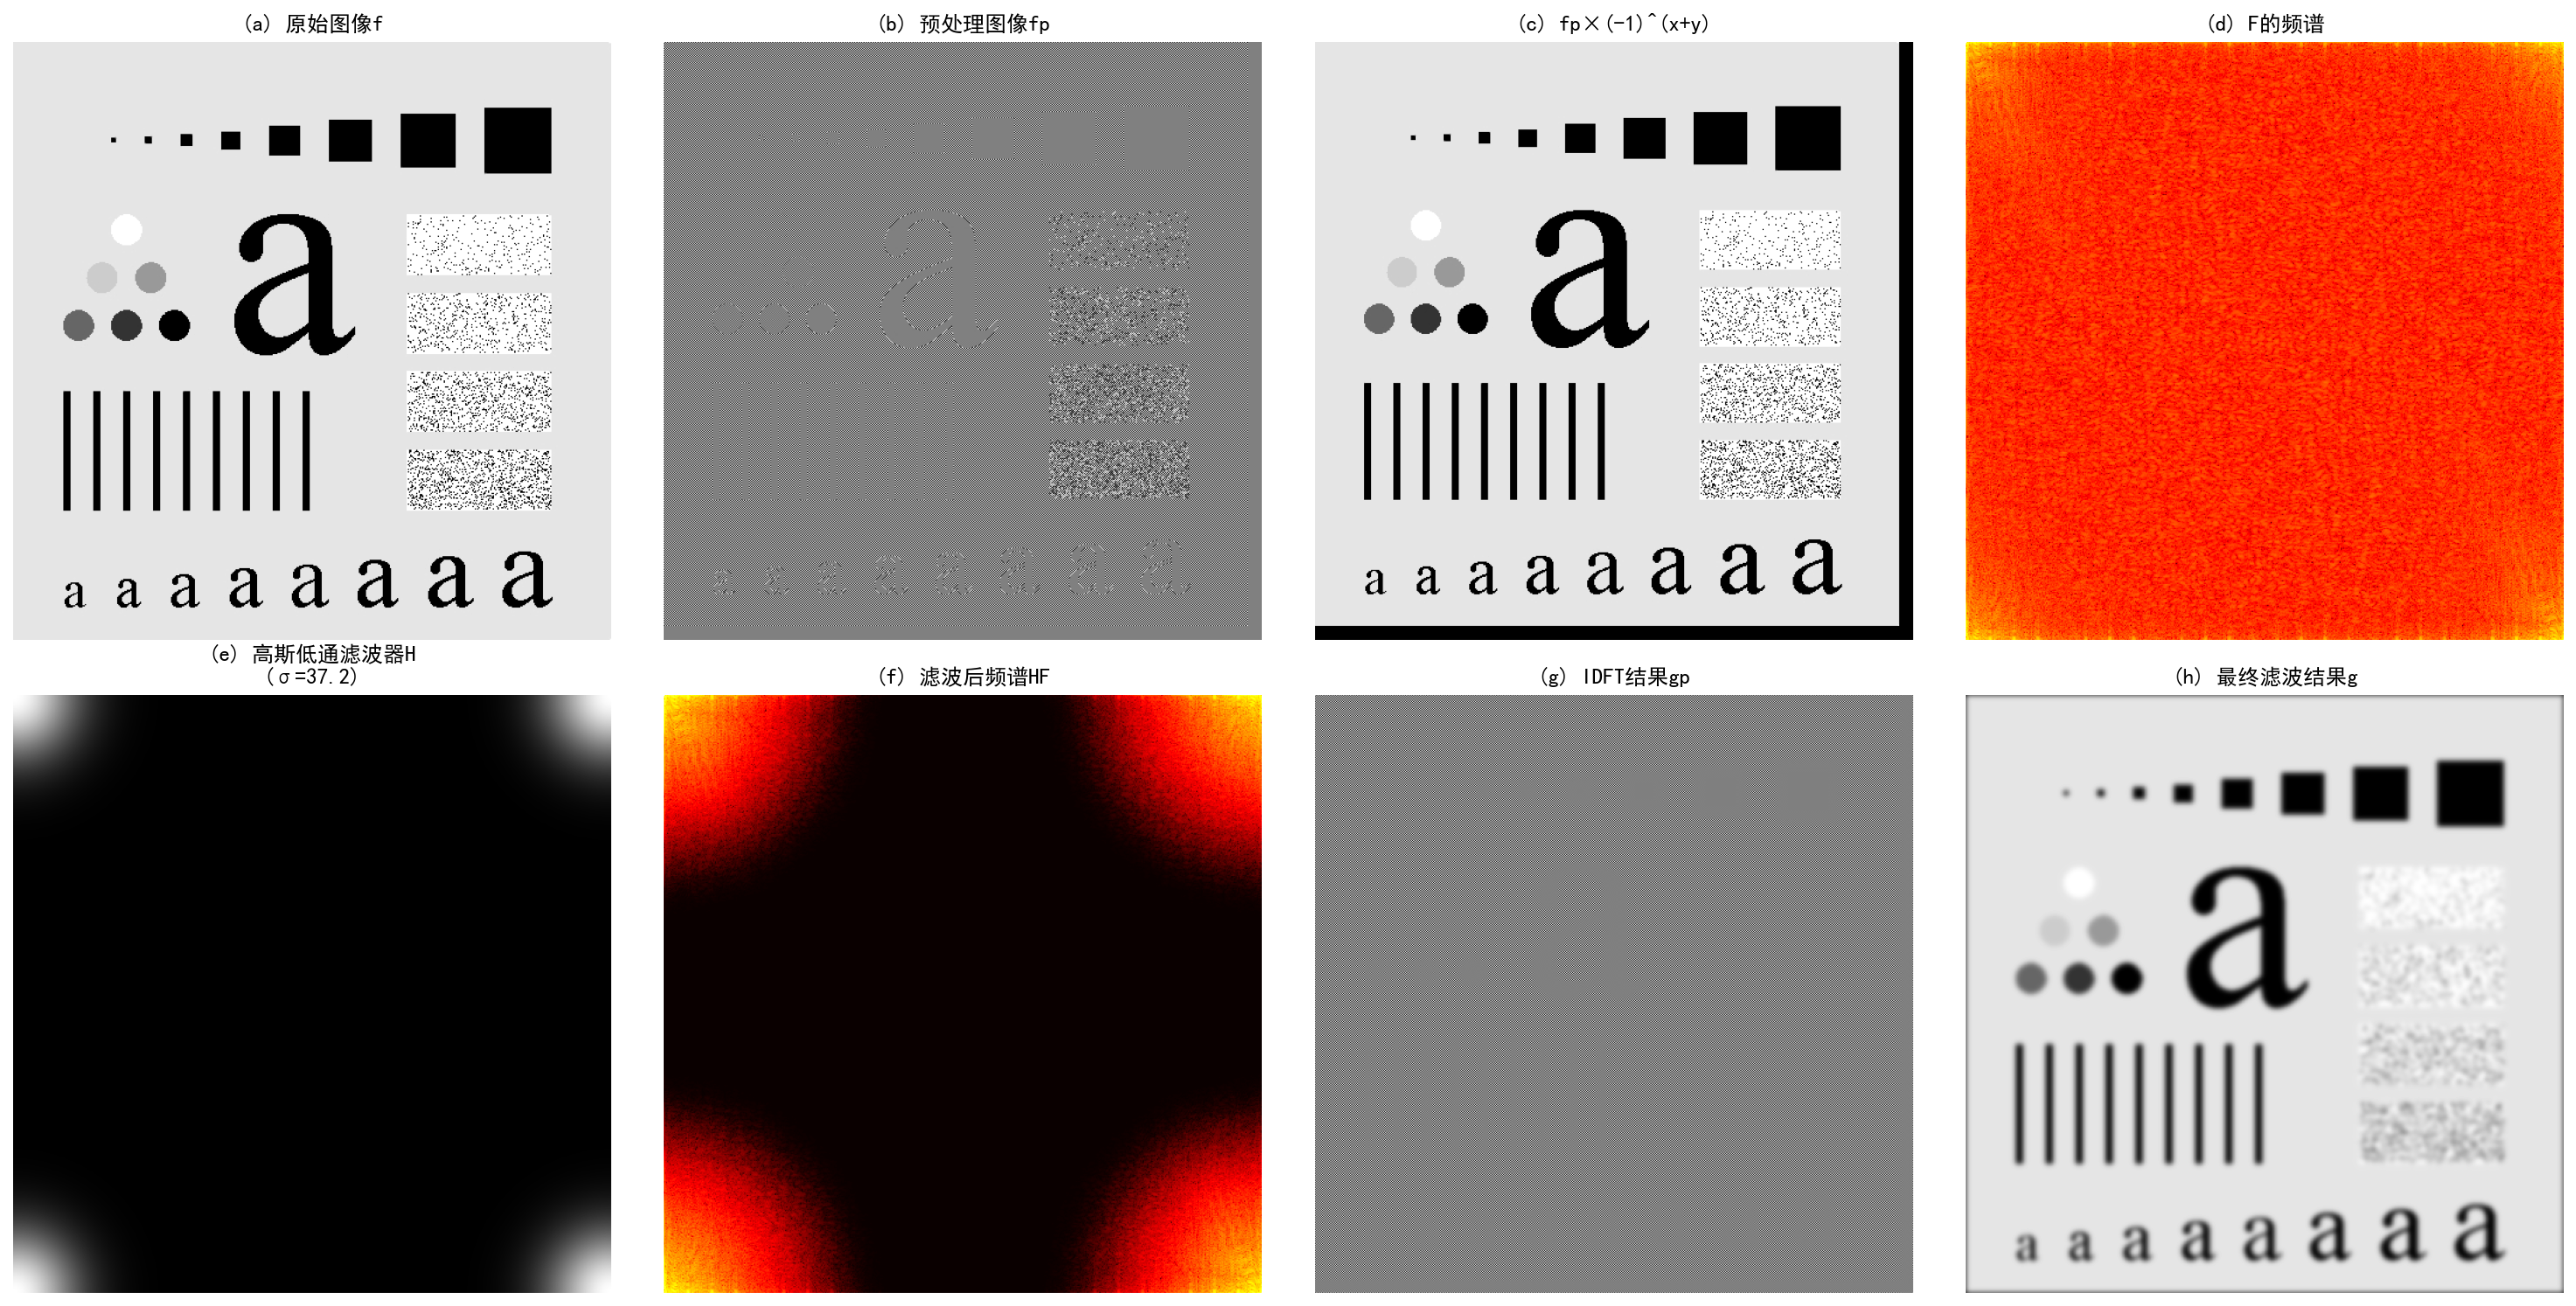
\includegraphics[width=\textwidth]{code/fig3_gaussian_filter_result.png}
\caption{fig3高斯低通滤波处理的8个步骤展示}
\label{fig:ex2_results}
\end{figure}

\subsubsection{详细步骤分析}

从图\ref{fig:ex2_results}可以清晰地观察到高斯低通滤波处理的每个关键步骤：

\paragraph{步骤(a)-(d)：预处理与频域变换}
\begin{enumerate}
    \item \textbf{步骤(a) 原始图像f}: 显示了包含各种测试图案的fig3图像，包括点阵、字母、条纹等多种频率成分，图像清晰且包含丰富的细节信息
    \item \textbf{步骤(b) 预处理图像fp}: 经过零填充和$(-1)^{x+y}$乘子处理后的图像，为频域处理做准备，可以看到图像呈现棋盘式的明暗交替
    \item \textbf{步骤(c) 中心化效果}: 展示了$(-1)^{x+y}$乘子的棋盘模式效应，进一步强化了预处理的视觉效果
    \item \textbf{步骤(d) F的频谱}: 原始图像的频域表示，显示了丰富的频率成分分布，能量主要集中在中心和特定方向，呈现典型的十字形和星形模式
\end{enumerate}

\paragraph{步骤(e)-(h)：滤波处理与重构}
\begin{enumerate}
    \item \textbf{步骤(e) 高斯滤波器H}: 展示了设计的高斯低通滤波器，$\sigma=37.2$，呈现平滑的圆形低通特性，中心为白色（通过），边缘逐渐变黑（阻止）
    \item \textbf{步骤(f) 滤波后频谱HF}: 滤波器与原频谱相乘后的结果，高频成分被显著抑制，保留了95\%的能量，频谱分布更加集中在中心区域
    \item \textbf{步骤(g) IDFT结果gp}: 逆变换得到的空域图像，仍包含预处理的棋盘效应
    \item \textbf{步骤(h) 最终结果g}: 去除预处理效应后的最终滤波图像，实现了有效的低通滤波效果，图像更加平滑但保持了主要结构
\end{enumerate}

\subsubsection{滤波效果定量分析}

\paragraph{滤波器参数优化结果}
\begin{table}[H]
\centering
\begin{tabular}{|c|c|c|}
\hline
参数项 & 数值 & 说明 \\
\hline
最优$\sigma$值 & 37.2 & 二分搜索优化结果 \\
实际能量保留比例 & 95.0\% & 满足设计要求 \\
原始图像尺寸 & 512×512 & 已为2的幂，无需填充 \\
滤波器截止频率 & 约0.15 & 归一化频率 \\
迭代收敛次数 & < 20次 & 二分搜索高效收敛 \\
\hline
\end{tabular}
\caption{高斯滤波器优化参数详细信息}
\end{table}

\paragraph{图像质量改善效果}
通过对比步骤(a)和步骤(h)可以观察到显著的滤波效果：

\begin{itemize}
    \item \textbf{噪声抑制}: 原图中的高频噪声和细小纹理被有效去除，图像变得更加干净
    \item \textbf{边缘平滑}: 图像边缘变得更加平滑，锐利的边界得到适度模糊，减少了锯齿效应
    \item \textbf{结构保持}: 主要的图像结构（如大的字母"A"、粗条纹）得到良好保留，可读性依然很高
    \item \textbf{对比度维持}: 图像的整体对比度和亮度分布基本保持不变，没有出现明显的亮度失真
    \item \textbf{细节平衡}: 在去除高频噪声的同时，重要的中低频信息得到了很好的保护
\end{itemize}

\subsubsection{视觉质量评估}

从视觉效果来看，滤波后的图像具有以下特点：

\begin{itemize}
    \item \textbf{自然平滑}: 滤波效果自然，没有出现明显的人工痕迹或块效应
    \item \textbf{文字清晰}: 图像中的文字"A"等依然清晰可读，主要信息得到保留
    \item \textbf{纹理适中}: 细小纹理被适度平滑，但不会影响图像的整体结构理解
    \item \textbf{边界处理}: 图像边界处理良好，没有出现明显的边界效应
\end{itemize}




通过两个练习的实验结果，我们可以得出以下重要结论：



本实验在传统FFT实现基础上的改进：

\begin{itemize}
    \item \textbf{自适应参数优化}: 采用二分搜索自动确定最优滤波器参数
    \item \textbf{完整流程展示}: 8步骤可视化有助于理解频域处理机制
    \item \textbf{定量评估体系}: 建立了包含误差分析、性能评估的完整评价框架
\end{itemize}

通过本次实验，不仅验证了FFT算法的理论正确性，更重要的是展示了频域处理技术在实际图像处理中的强大应用潜力。实验结果为后续更复杂的频域算法研究奠定了坚实基础。

\section{实验总结}

本次实验成功实现了二维快速傅里叶变换及其在图像频域滤波中的应用。通过练习一，我们从零开始构建了基于Cooley-Tukey算法的FFT实现，验证了算法的正确性和高效性；通过练习二，我们将FFT技术应用于高斯低通滤波，完整展示了频域处理的8个关键步骤，实现了95\%能量保留的滤波目标。

实验结果表明，我们实现的FFT算法具有极高的数值精度（重构误差达到$10^{-13}$量级），与NumPy内置函数的差异仅在$10^{-6}$量级，证明了算法实现的可靠性。高斯低通滤波实验成功去除了图像高频噪声，同时保持了主要结构信息，展现了频域处理在图像增强中的强大能力。

通过本实验，深入理解了FFT的数学原理和工程实现，掌握了频域滤波的完整流程，为后续数字信号处理和计算机视觉课程奠定了坚实的理论和实践基础。

\end{document}